% EPL master thesis cover template
\documentclass{eplmastersthesis}

% help package for todo
\usepackage{xargs}                      % Use more than one optional parameter in a new commands
\usepackage[pdftex,dvipsnames]{xcolor}  % Coloured text etc.
% 
\usepackage{hyperref} % for url and so on
\usepackage[colorinlistoftodos,prependcaption,textsize=tiny]{todonotes}
\newcommandx{\unsure}[2][1=]{\todo[linecolor=red,backgroundcolor=red!25,bordercolor=red,#1]{#2}}
\newcommandx{\change}[2][1=]{\todo[linecolor=blue,backgroundcolor=blue!25,bordercolor=blue,#1]{#2}}
\newcommandx{\info}[2][1=]{\todo[linecolor=OliveGreen,backgroundcolor=OliveGreen!25,bordercolor=OliveGreen,#1]{#2}}
\newcommandx{\improvement}[2][1=]{\todo[linecolor=Plum,backgroundcolor=Plum!25,bordercolor=Plum,#1]{#2}}
\newcommandx{\thiswillnotshow}[2][1=]{\todo[disable,#1]{#2}}

% Fill in here the information: title, student name, speciality, jury members
\title{Privacy Aware Sharing of IOCs in MISP}	% Master thesis title
%\subtitle{Subtitle (optional)}			% Optional subtitle
\author{Charles \textsc{Jacquet}}	% Student name
%\secondauthor{Firstname \textsc{Lastname}}	% Second student name if applicable
\speciality{Computer Science and Engineering}		% Speciality (use one of the following options):
										% Biomedical Engineering
										% Chemical and Materials Engineering
										% Civil Engineering
										% Computer Science
										% Computer Science and Engineering
										% Electrical Engineering
										% Electro-mechanical Engineering
										% Mathematical Engineering
										% Mechanical Engineering
										% Physical Engineering
%\options{Option(s)}		% If required by program commission mention options
\supervisor{Ramin \textsc{Sadre}}	% 1st supervisor name
%\cosupervisor{Firstname \textsc{Lastname}}	% 2nd supervisor name if applicable
\readerone{Antoine \textsc{Cailliau}, Alexandre \textsc{Dulaunoy}}		% 1st reader name
\readertwo{William \textsc{Robinet}}		% 2nd reader name
\readerthree{François-Xavier \textsc{Standaert}}	% 3rd reader name
\years{2016-2017}	% Academic year

\begin{document}

\maketitle					% To create front cover page
\thispagestyle{empty}		% To suppress header and footer on the back of the cover page


\begin{abstract} 
Malicious software (malware) are plaguing this computer age. But how to avoid them ?
An actual solution is threat information sharing where companies share lists of Indicators Of Compromise (e.g. IPs, mail addresses, urls, malware hashes and so on) with each other.
An interesting tool is the MISP (Malware Information Sharing Platform), a platform that allows companies to share these IOCs but also malware analysis.
Sometimes, the information is somehow confidential, but still interesting to be shared, thus we need to find a way to share these secret information without disclosing them entirely.
The goal of this master thesis will be to analyze the state of the art and to implement different solutions working with MISP in order to compare their performances.
\end{abstract}
\chapter{Introduction and State of the Art}
\section{Interaction with this Latex Document (To be removed)}
In order to facilitate comments, I've added some new commands explained by\footnote{http://tex.stackexchange.com/questions/9796/how-to-add-todo-notes}:\\
\begin{itemize}
\item unsure => What I need to check
\item change => What have to be modified
\item info => Add simple comment
\item improvement => Indicate a possible improvement
\end{itemize}

\section{Introduction}
In the last report of the Ponemon institute, we can see that the estimated cost of annual data breaches for 384 companies in 12 countries\footnote{United States, United Kingdom, Germany, Australia, France, Brazil, Japan, Italy, India, the Arabian region (United Arab Emirates and Saudi Arabia), Canada and, South Africa} is about \$4 million. Moreover, 48\% of theses breaches are due to malicious and criminal attacks.\\
Taking that into account, the damage cost per capita is about \$170 only for malicious and criminal attacks. \\
Beside that, Cybersecurity Ventures predicts the global annual cybercrime costs will grow from \$3 trillion in 2015 to 6\$ trillion by 2021.\\

We thus need to improve our computer defenses and make them to learn continuously about new appearing threats. Moreover, they should be aware of new threats faster than simple malware detectors or anti-viruses. This is why a new kind of security levels appeared and is called threat sharing. As soon as an organization find a malware, they can prevent others to be compromised just by letting them know about the threat. \\
Unfortunately, this is not enough as, theses informations, here and after called IOCs, are often considered as confidential because revealing them, can reveal damaging information for the companies.\\
We thus need to find a way for \textbf{sharing} information without \textbf{giving} the information. And I will try to explain the meaning of this sentence in the report's body. But, for now, we can say that this master's thesis is on finding a "more secure" way of sharing information. More precisely, if we attempt to create an encrypted database of these IOCs, the idea would be to slow down as much as possible a brute force attack for someone who has complete access to the database while still making this database useful for the targeted user.\\

I've decided to organize the work the same way I've discovered and implemented things. The first chapter will thus be on defining the tools an vocabulary that will be used. I'll be continuing this chapter with a state of the art that made me understood the domain and the limitation that I was going to face.\\
Afterwards, I'll spoke about the implementation ideas I've got, by highlighting theirs strengths and weaknesses. While the third chapter will really be about my implementations, my choices on the system but not only on the way I've implement things but also the library I've chosen.\\
The next one will be an analyze of the implementation supported with different benchmarks.\\
Finally, I will conclude on my work with some possible improvement and future work but also by concluding on every thing that I've discovered.

\section{Indicator of Compromise (IOC)}
If there is a crime, detectives can come and look for clues. What make it happened, why did it happened and how did it happened. The what and why questions can be interesting in order to avoid this crime to happen again while the last one but not the least one, the how can be used to compare this crime with other similar ones.\\
This idea of being able to compare them is really interesting as seeing the clues of only one place can be not enough while there could be enough clues if we succeed in gathering the whole set clues.\\
This is exactly the same idea here, even if the attacker try to minimize its traces, there are always some. They can be email addresses, IP addresses, malware, url and so on.\\
The idea, is then to use these traces to trigger alarms on other computer system as soon as they are seen. This means that the same attack is perhaps happening again but and this is the reason why we call them Indicator Of Compromise.


\section{Cyber Threat sharing}
\improvement{Perhaps add the information coming from the Guide + historical inforamtion}


\section{MISP and Threat Sharing}
I've introduce the idea of malware sharing to defend our computer systems against digital threats and attacks. But MISP is not the only platform to do so, the more current onces are DShield, Critical Stack’s Intel, Microsoft’s Interflow, AlienVault’s Open Threat Exchange, ...\\
But here I focused on the MISP project which is, as said on their website, an open source software solution for collecting, storing, distributing and sharing cyber security indicators and threat about cyber security incidents analysis and malware analysis. MISP is designed by and for incident analysts, security and IT professionals or malware reverser to support their day-to-day operations to share structured informations efficiently.\\
A recent paper on MISP \cite{wagner2016misp} had been published this year and could be interesting if your are searching to have a better understanding of the underlying system.

\subsection{History}
Christophe Vandeplas started the project as he was tired of the way IOCs were shared (email, pdf, .. ). Thus, he created a cakePHP website as a proof of concept and manage to convince the Belgian Defense (where he was working) that the project was worth to work on. They even allowed him to work on it during his work-hours. The project continued to move forward and now, Andras Iklody is the lead developer of the MISP project and works for CIRCL.\\

\subsection{The Basics of Misp}
The basic idea of misp was thus to create an IOC database, for example, if we have two IOCs for the same attack, let's say "IOC@malware.mail" and "192.168.16.2". We are interested to  keep the information that there has been an attack that can be recognized thanks to these two IOCs. That is why they have created events (which is much more general than the term attack that I've been using) and they use these IOCs as the attributes of this specific event. \\
Then thanks to this idea, we can analyze the event and even make correlations with other events if they possess similar IOCs.

For clarity concerns, attributes are divided into 13 categories where they are again dived into types. As MISP is no more only targeting malwares, it is interesting to notice that we can also see categories like Financial Fraud. More standard ones are Network Activities, Antivirus detection, Artifacts dropped, and so on.\\
All the category and types can be found on this web pages \url{https://www.circl.lu/doc/misp/categories-and-types/index.html}

One other really interesting feature is sightings. When an IOC is referenced, we know that it has been seen by someone, but it does not confirm that the IOC is really related to that particular event and is not an error. Moreover, what says that the if an IP address is an IOC today that it is going to be the case in 3 months ? \\
Sightings is thus the solution to this problem as we can monitor an IOC, knowing if it has been seen at other places, and if they are still relevant.


The two important things on the sharing strategy that I want to point out are the MISP instances and communities. The first one is easy to understand, MISP is an open source project which means that everybody can decide to run a completely isolated MISP instance for its own needs like a company for storing its own confidential data. Besides that, that does not mean that the instance must be isolated, they have implemented a way to share information between these instances. While the second one is a good property of an instance. When we are connected to MISP as a user, we are connected thanks to the organization that we belongs. Then, the organization can choose to share or not to share their events/attributes with other communities or even with other instances. \\ 

Now, as a good open source project, a whole ecosystem has been created around and more and more companies are using it.\\
MISP become a really good IOC database with automated correlation system. We can even create correlation graphs to see how different events are connected together what helps a lot for the threat analyses.\\
Beside all that, a lot of different tools like a python client library are available on their repository : \url{https://github.com/MISP/}.\\
They have also improved added a lot of value to the web api like the ability of exporting the attributes in a lot of different format and some that can directly be used in IDS.\\

\subsection{My Settings}

There is thus a lot of things to understand in order to work with misp. That's why they are giving trainings (I've followed one during the summer holidays) and that they make available a misp training virtual machine.\\
At the beginning, I've started to work directly with the private instance of MISP hosted by CIRCL but, every time that I was working, I needed to have a really good web connection to connect myself and to download all the data. That's why, I have finished by downloading the virtual machine. But, as I was going to work on my computer and I didn't want to be stuck to work inside the virtual machine, I've done some modifications.\\
The mysql database wasn't accessible from the outside of the virtual machine (which is completely understandable as they don't want anyone to have a direct access to the complete unprotected database) and I've also got some network problems.\\
The first step was that my virtual machine running on virtualbox was using the virtual vboxnet0 interface and was using, as its IPv4 address, 192.168.56.50. The problem was that, normally it works without problems but my computer does not know about the subnetwork. I thus had to add an ip in the right range by using the command :
\textbf{ip add add 192.169.56.2/24 dev vboxnet0} .\\
I'm also sometimes using a second virtual machine to work with and on this virtual machine, I've configured two network interfaces, the first one was to have an internet connection while the second one was the vboxnet0 interface.\\
For simplifying the use of the vbox interface, I've configured my network to automatically add an ip in the right range (/etc/network/interfaces). This is the addition on the basic configuration:
\begin{verbatim}
auto eth1
iface eth1 inet static
address 192.168.56.1
netmask 255.255.255.0
\end{verbatim}
 
After that, I was able to contact the virtual machine via the network but it wasn't enough to have a mysql access. For that, as the misp virtal machine was only accessible from the vboxnet0 interface, it was a problem to create external access for all ip addresses with only a small password protection.\\
The first step for that was to modify the configuration file (/etc/mysql/my.conf) where I've juste commented the "bind-address 127.0.0.1" line.
The next step was to create a user with the rights from the outside. For that, I've connected myself to the database as the misp user and I've added the user:
\begin{itemize}
\item[•] mysql -uroot -pPassword1234 
\item[•] CREATE USER 'username'@'\%';
\item[•] GRANT ALL ON *.* TO 'username'@'\%';
\end{itemize}

Once done, I could continue to program more easily and create some tests as I could control the whole available set of data. For testing when the code was modified, I had used a really small set of data. \\
But speaking about testing, I didn't do any automated test as the system requests some connections, It was not easy to generate them. \improvement{Do automated test !}

\subsection{Illustrations}
There is nothing better to illustrate all that than real screen shot of the web application. But, it raised the question of what can be shared in MISP?\\
For example, Am I allowed to show screen shot of data from MISP without any risk ?\\
To respond to that question, I need to introduce the Traffic Light Protocol (TLP) that was created in order to facilitate information sharing by defining the authorized level of disclosure. And thus, it can be used to know what can be shared with a specific audience.\\
This protocol is defined by FIRST in \cite{FirstTLP} but also in this NIST cyber threat information sharing guide \cite{johnson2016guide}.\\

Knowing that, I know that I can share the data from the virtual machine that I have explained in the previous section as the default OSINT feed is TLP:WHITE. Which means, according to FIRST, that the disclosure is not limited: \\
Sources may use TLP:WHITE when information carries minimal or no foreseeable risk of misuse, in accordance with applicable rules and procedures for public release. Subject to standard copyright rules, TLP:WHITE information may be distributed without restriction.\\

The first pages (after the connection) of the web application is a list of all latest events on figure \ref{webevents} (notice the tlp:while appearing in the Tags):

\begin{figure}[!h]
	\begin{center}
		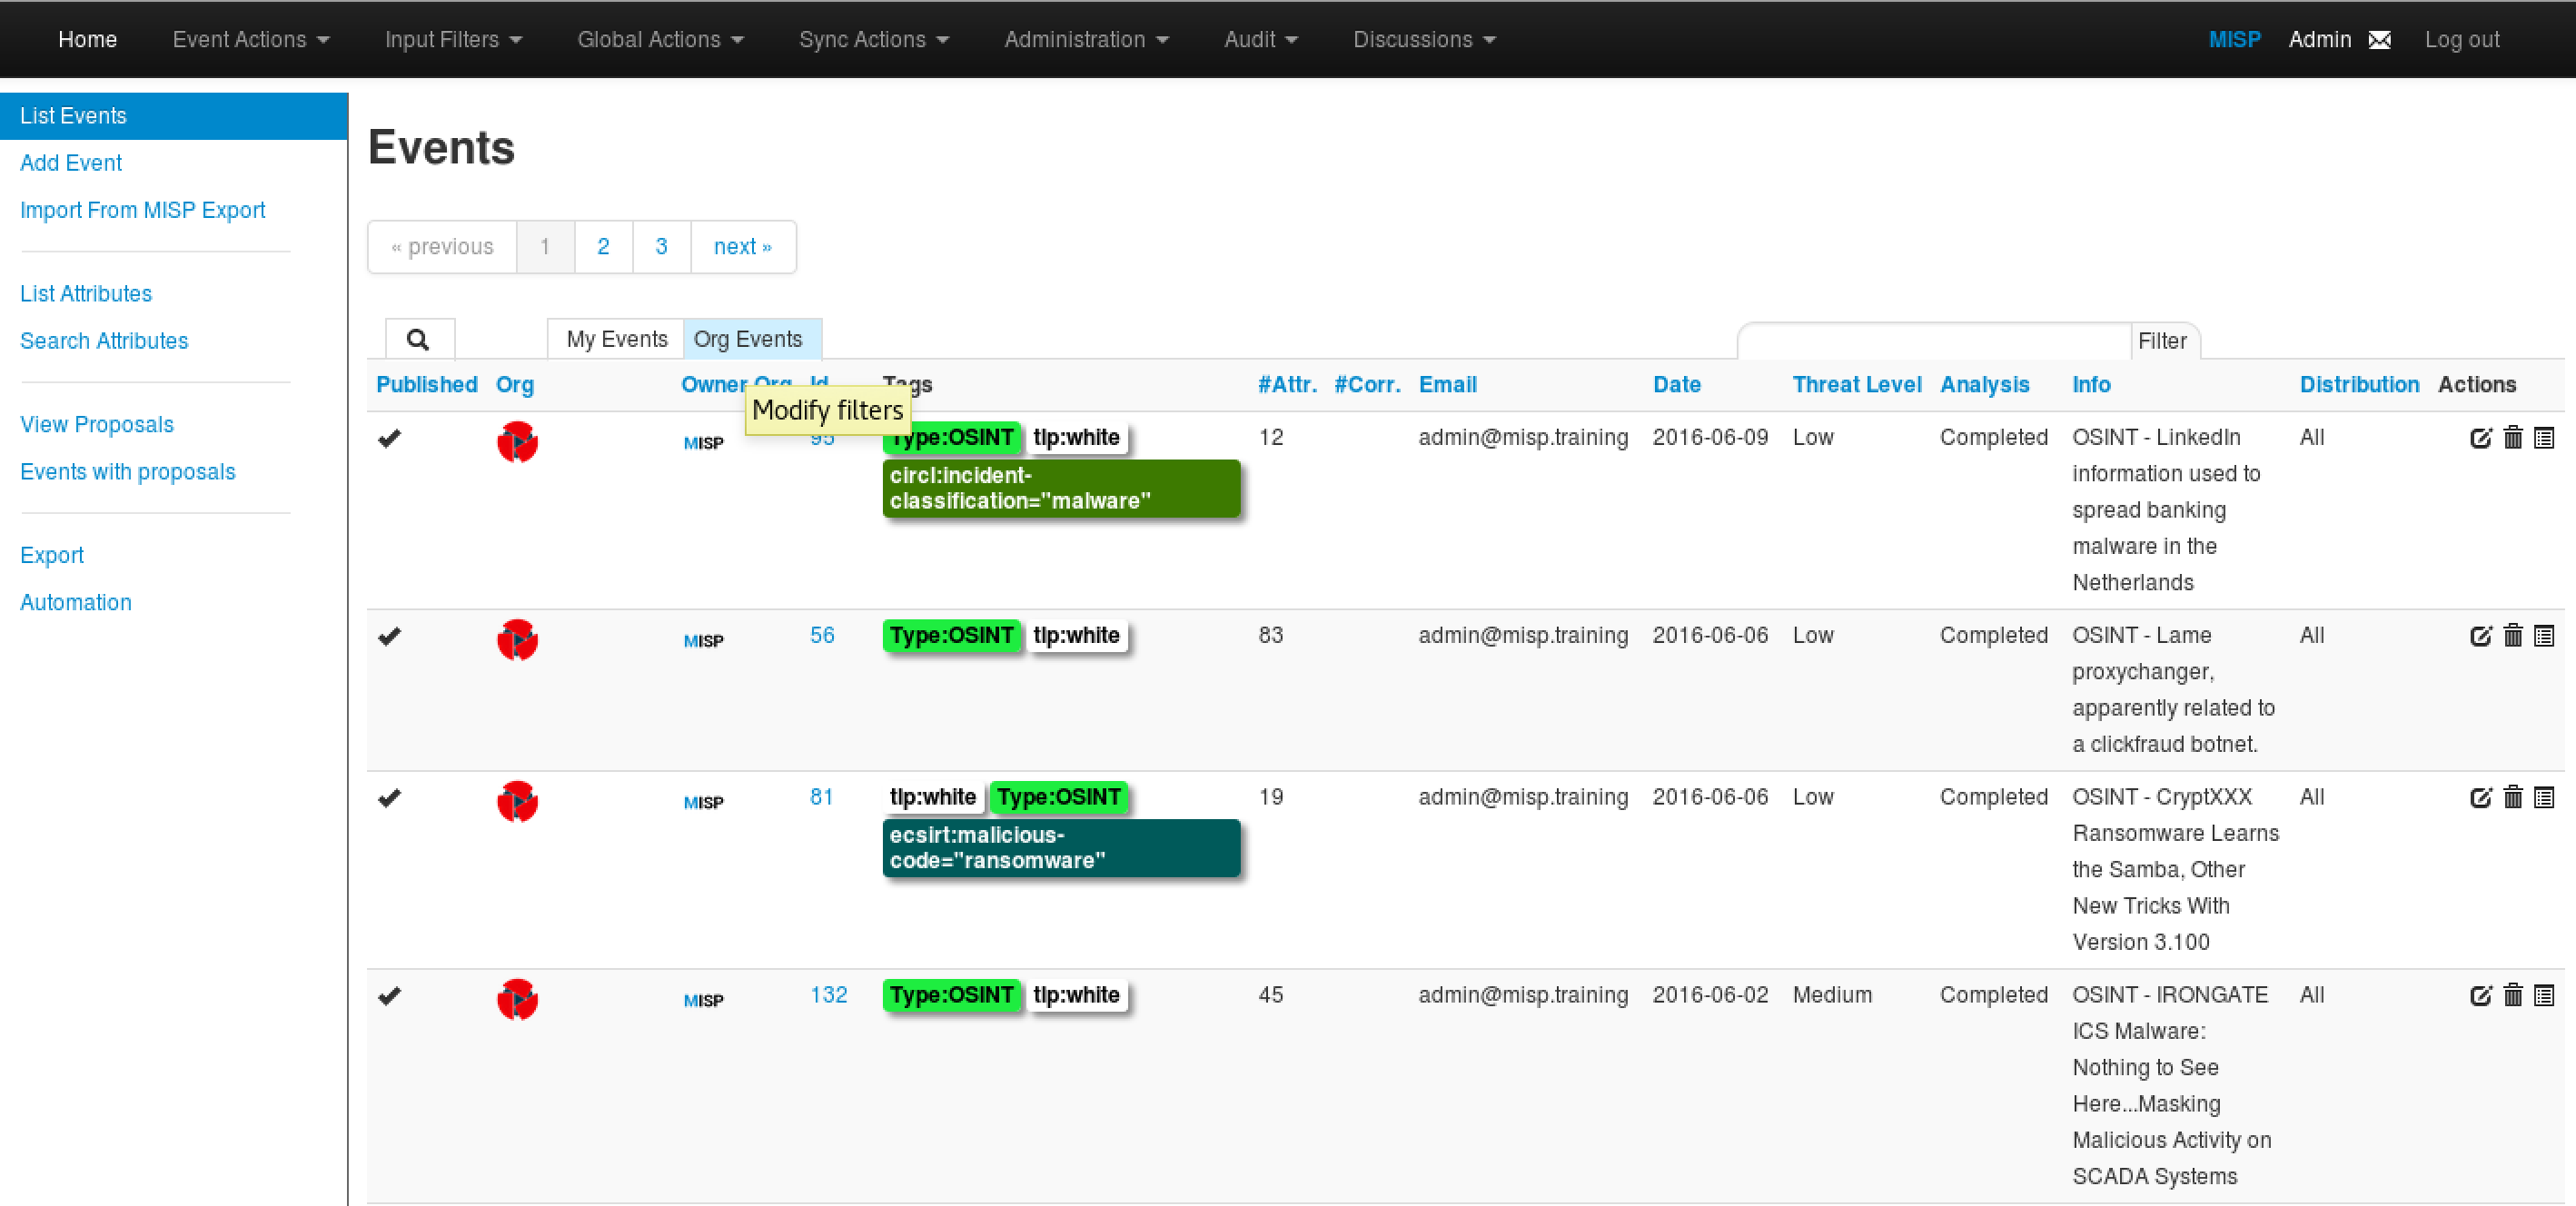
\includegraphics[scale=0.32]{res/webEvents}
		\caption{MISP : List of events}
		\label{webevents}
	\end{center}
\end{figure}


Then, by clicking on an event, we can get information on it \ref{webevent}:


\begin{figure}[!h]
	\begin{center}
		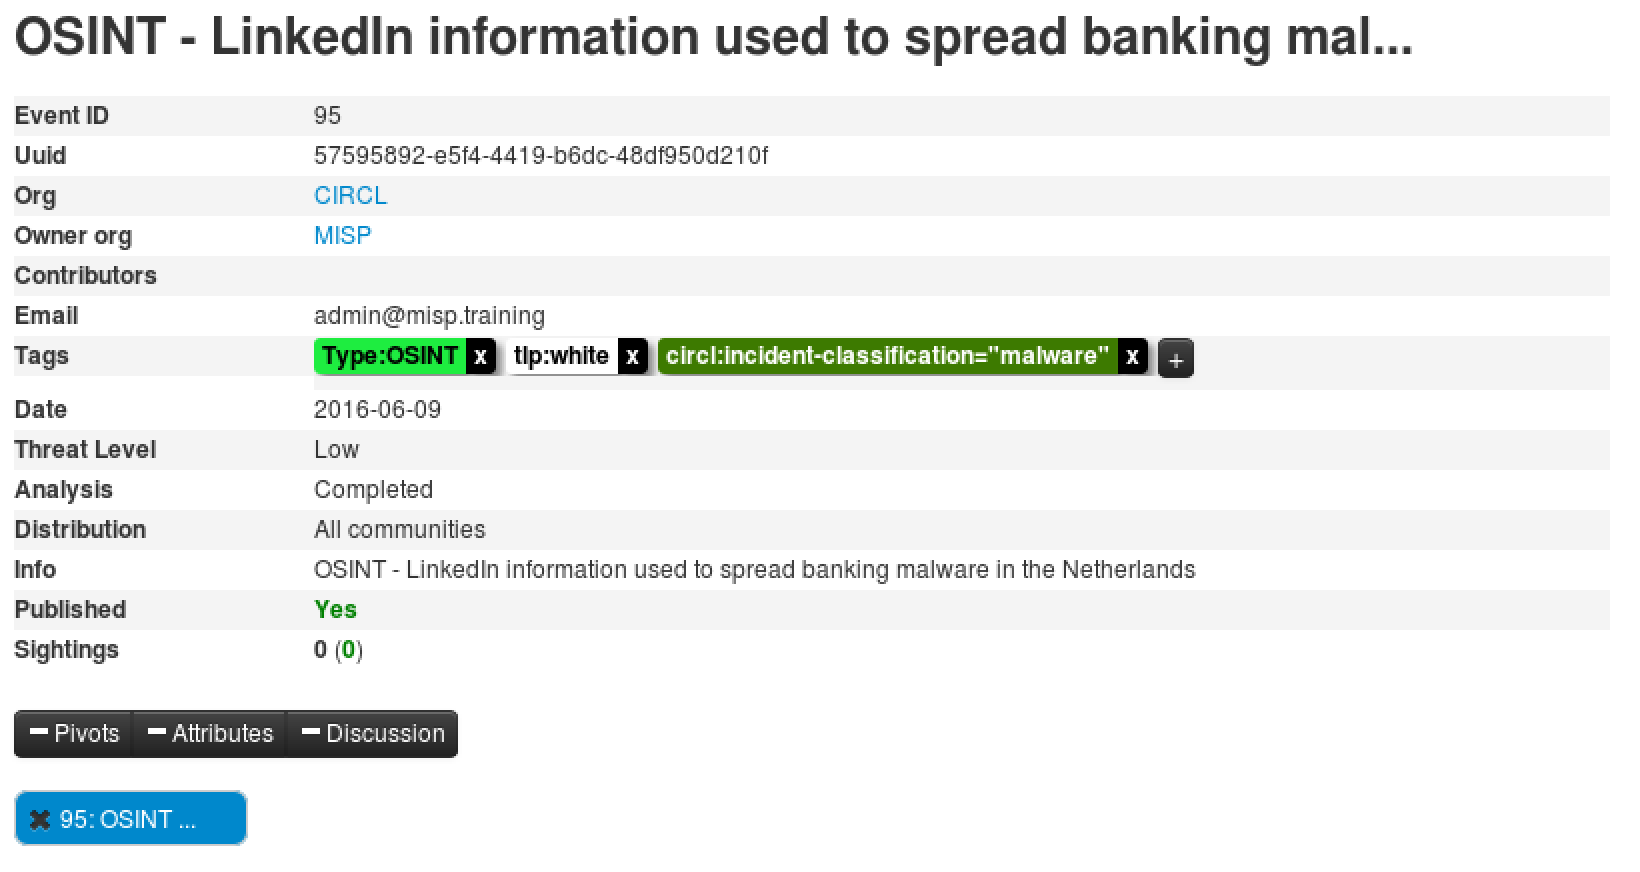
\includegraphics[scale=0.35]{res/webEvent}
		\caption{MISP : Specific information on the event}
		\label{webevent}
	\end{center}
\end{figure}


As well as the attribute list \ref{webattributes}:
\begin{figure}[!h]
	\begin{center}
		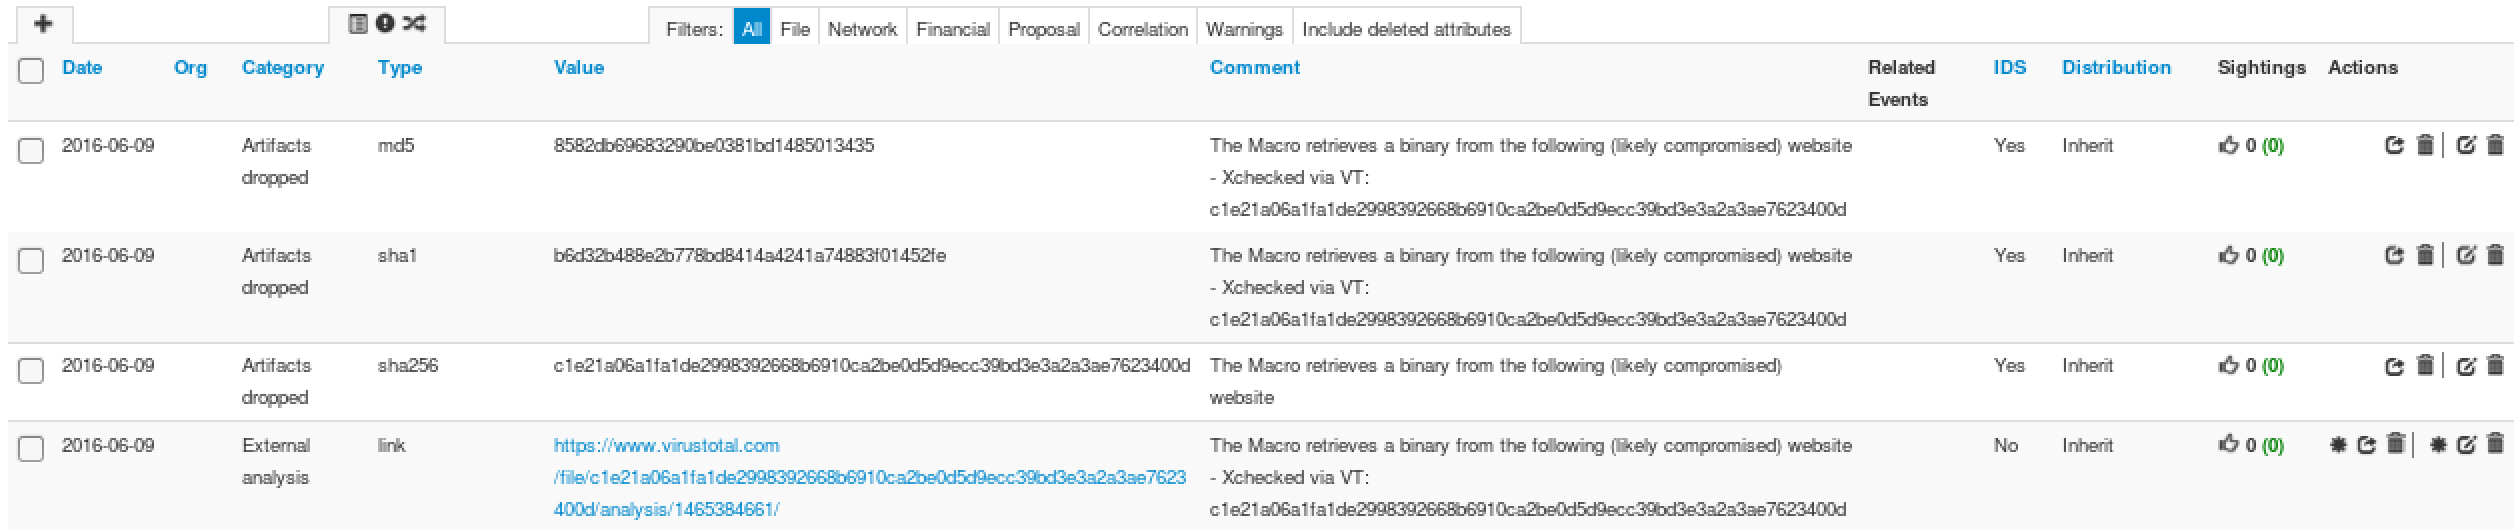
\includegraphics[scale=0.35]{res/webAttributes}
		\caption{MISP : Attributes of the event}
		\label{webattributes}
	\end{center}
\end{figure}

And the last thing that I want to show is one of the way of showing the correlations with other events and is called the correlation graph \ref{webcorrelation}:
\begin{figure}[!h]
	\begin{center}
		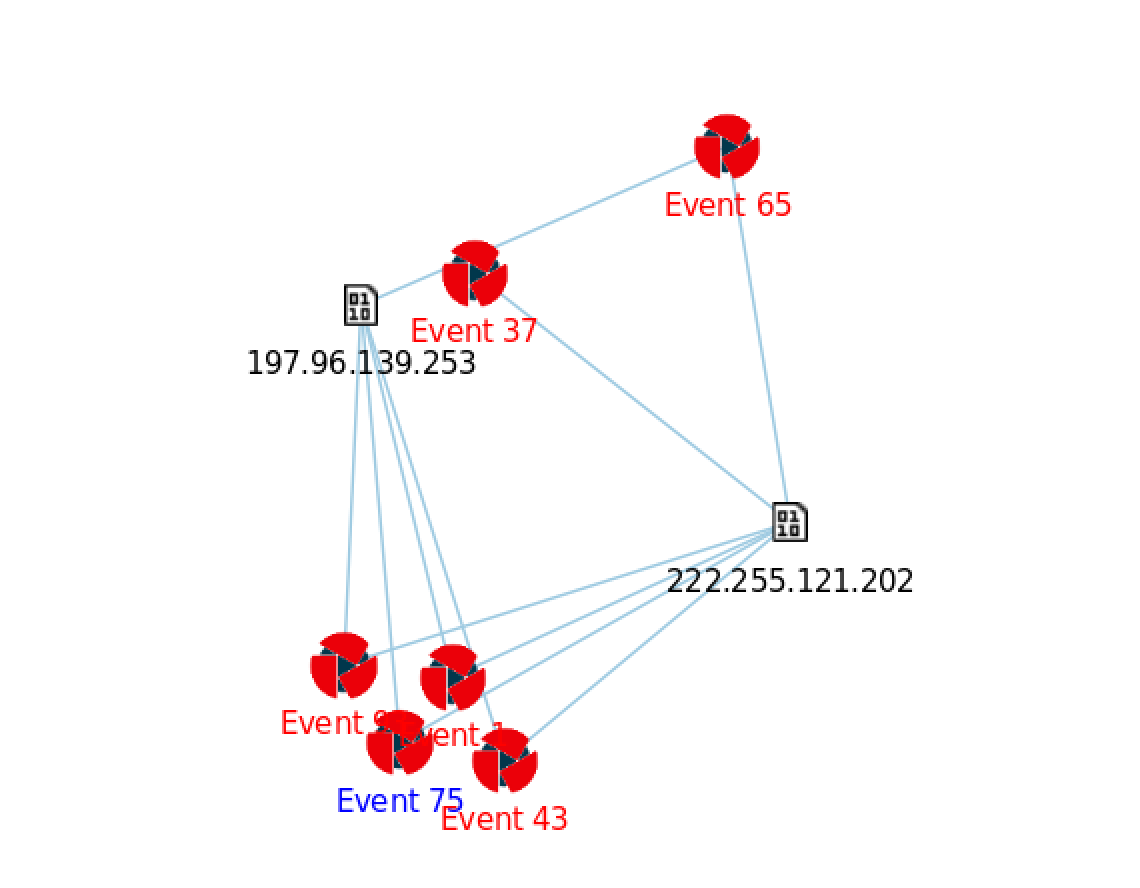
\includegraphics[scale=0.35]{res/webCorrelationGraph}
		\caption{MISP : Correlation graph for an event}
		\label{webcorrelation}
	\end{center}
\end{figure}



\section{Information Sharing State of the Art}
The idea of this section is to sum up all different articles read at the beginning of the master thesis. These are articles are linked to the subject but sometimes not directly but helped me to the understanding of the subject, and especially to discover ideas to create some possible solutions.\\
These articles can be divided into some sections, the first one is data sanitization, this is quite interesting even if it could not be applied in our case (as explained in a later section).\\
Then we have articles on confidencial database and S2P computations \change{I have to complete these parts with articles}
\change{Add the explaination on the article on ip sharing at the end}
\change{Add also a section of other kind of detection system like the DNS one of http://conferences.sigcomm.org/imc/2015/papers/p197.pdf}

One of the first articles that presents some concerns about privacy in sharing security alert is \cite{lincoln2004privacy}.
More precisely, they were concerned about protecting site-private topology, proprietary content, client relationship and site defensive capabilities or vulnerabilities.\\
This was done in 2 steps, the first one, called data sanitization consist in removing confidential data and remove useless information. We don't take the chance of revealing information to an attacker if this one is not needed.\\
The second one is the correlation/aggregation work were alerts are linked together for analyses purpose.\\
Before explaining deeper how they sanitize data, it's interesting to first focus on how they get them!\\
 They have used three different categories:
\begin{itemize}
\item Firewalls : They consider all "deny" as a possible attack
\item IDS : They remember logs of attacks that the IDS has found
\item Anti-viruses softwares : gives also some interesting logs
\end{itemize}
They based their analyses on data coming from DShield and Symantec's DeepSight.\\

Let's come back on data sanitization, as already explained, we first remove all useless information, then, we can hash all confidential data!\\
The advantage of leaving this work to the company is to avoid the need of trust on the repository.\\
This technique is quite well working if, the data has a certain size. But, on the other hand, it's not useful for IP addresses, if an attacker is targeting a company, it has to precompute only 256 or perhaps 65536 IP address hashes. Thus this is not brute force resistant!\\
For each alert, we have two different IPs, the source IP (ip\_src) and the destination IP (ip\_dest). We can classify all these IPs in two categories:
\begin{itemize}
	\item Internal IPs : IPs that belong to the company
	\item External IPs : IPs external to the company
\end{itemize}

The first category is, of course, the one that we want to protect and in order to do so, these IPs are hashed with a HMAC algorithm. While the second one is hashed by a simple hash algorithm like SHA-1.\\
The result is that we can compare all SHA-1 hashed IPs together while only companies can decrypt their own internal IP addresses.\\
It is an efficient technique as they receive millions of IPs all the time. And, as the attacker is not able to see if the IP is hashed by HMAC or SHA-1, he has to test all hashed IPs against a precomputed table which is not feasible.\\
They are also using another set of protections like the randomized threshold for publication of an alert but I'm not going to spend time on it.\\
In sanitization, the also round all timestamp to the nearest minute in order to add some uncertainty!\\
The second step is the correlation, they spoke about historical trend analyses, source/target-based analyses and event-driven analyses but some other articles are more interesting for the correlation principle, thus I'm not going deeper in it.\\

Then, \cite{xu2005privacy} was also working on confidential data sharing starting from the first article, but they came up with a new interesting idea, instead of hashing confidential data, why not generalize it and do probabilistic correlations.\\
(They also used a technique to create probabilistic attack scenario which is a set of alerts that are put together to create a bigger attack).\\
\textbf{Guided alert sanitization with concept hierarchies:}\\
For example, if we have an IP 192.168.1.123/32, we can generalize it to 192.168.0.0/16.\\
The depth of the generalization is chosen thanks to the entropy or the differential entropy technique explained in \cite{cover1991elements}.
\\
\textbf{Alert Correlation:}\\
They focused on defining similarity functions between sanitized attributes and building attack scenarios from sanitized attributes
\\

This article was interesting for seeing a technique of data obfuscation. And then to create correlation analyze but, it's difficult to apply that technique in order to create a database of confidential data !
\\

I've explained some solutions that can be applied to IP addresses or file (just hashing them). But, what if we could do the same with all network packets and still getting some privacy!\\
That's the goal of \cite{parekh2006privacy} ! Today, it's not enough to analyze IPs, URLs and so on. We need to go deeper in it, that's why they propose a technique based on the byte distribution of the packets.\\
They used PAYL and Anagram \cite{wang2006network}, systems that they have created and which are really useful in these analyses.\\

But, if we have some confidential information, instead of sharing with everyone, we could simply select organizations with which we have benefit to share. But for that, each organization needs to have their database and to be able to do some secure two-party computations.\\
The interest is to get some metric, for example, if there are only IPs in the databases, if we can get the intersection, and if the cardinality of this intersection is non-negligible, we know that it could be interesting to share with them!\\
The paper written by Freudiger and al \cite{freudiger2015controlled} focused on this problem by working on a DShield dataset. They've experimented some strategies to know if it could be useful to share or not with another company. And then, they also experimented to share the whole dataset of the company, only the data set linked to the intersection just found or only, the intersection (just to get a rough idea of what they have in common ... ).\\
Their conclusion were intuitively expected but still interesting :
\begin{itemize}
\item More information we get on an attacker, the better the prediction are !
\item The chosen collaboration strategy has a really big impact (some of the strategies are really useless)
\item Collaboration with companies improves not only the predictions but also removes a lot of false positive.
\item Sharing only about common attackers is almost as useful as sharing everything!
\end{itemize}

\section{Sum up}
The first idea imagined was a simple proof of work database. But, even if it's an interesting way of remembering and sharing data while avoiding total disclosure of the data set. It has a big disadvantage as well, we cannot really use data for analysis since an enormous amount of computation is needed to get all information, and then, how could we compare them?\\
Thus, I had to go deeper and to look into scientific papers. As there are not a lot of information about MISP in this kind of literature \info{there is now a new paper \cite{wagner2016misp}}, I had to find another starting point. The one I found was DShield. This is also a kind of sharing platform. Even if the way they get or use data is quite different, the general concept is the same or at least for my approach.\\
Then, I could find a lot of techniques in order to generate blacklists, detect event correlations and protect companies with it.\\
I also found privacy concerns about sharing data. And thus, a lot of separate techniques. For example, if there is privacy problem with sharing files, we can simply hash them. It's not possible to brute force in order to get back the starting file but, for IP addresses, since in general, there are only 256 or 65536 IP addresses for a specific company, we could create a table with all possible hashes and test them all!\\
That's why it was interesting to see how they handled these problems but, as these techniques were built in view of a special purpose, they have some disadvantages for us. \\
For example, if we need to store the whole data set, proof of work database with bloom filter to make some analyze could be enough but if the idea is to make correlation between data, this idea is not good enough and we need to focus on other techniques.\\
But on the other hand, an other widely used technique is data sanitization as seen with articles examples. But again, some problem arise when we want to analyse data. Wath could we do with an ip where the most signicant bit could have been modified by noise. Or with an ip without modified with concept hierarchies ? \\
Sanitized data loose all the information needed in these process so we need to find one another technique.\\
That's why I created a set of questions that could help me to know what I need to focus myself on :
\begin{itemize}
\item When we spoke about privacy, do we speak only about data privacy or also about source anonymity ? \\
$\Rightarrow$ Here the question is not to know who had seen it before, but just to determine what is going on. We only need to have like a hashstore of data to be sure that data cannot be recovered ! But we need to find a way to be sure to securely share IPs !
\item How to define the sate of an IOC ?\\
 $\Rightarrow$ This is done in misp and has no impact on my work
\item How MISP is used by companies? What is really the difference with DShield ?\\
$\Rightarrow$ DShield is used just by getting automatically a lot of data in order to discover as soon as possible all big attack in order to block them ! While MISP is to analyze event and share it with other companies
\item In MISP, event correlations are done but, are they working on attack scenarios ?\\
$\Rightarrow$ I don't think so, but I forgot to ask this question
\item Are misp allow some groups (collaboration) to know the intersection of their attributes with other group in order to know if it's worth to share ?\\
 $\Rightarrow$ No, at least not for the moment !
\end{itemize}

\section{Useful Cryptographic Functions}
\improvement{Todo}

\section{On what I worked}

We have a data set of malicious data, IOCs, events and we want to share them. And it is already done by the MISP project. But now, if we want to distribute these information to every one?\\
It would be really nice, every computer specialist could check on computers to discover infections, problems and moreover fix it thanks to previous analysis contained on MISP. But there is a problem, some information are confidential and we need to have some privacy concerns while sharing. \\
Actually, it is quite easy to understand this fact. If a company have data, they have it so they don't want to share it! Even more if it can be confidential but in the other hand, if they can avoid infection, or detect it with information from other companies, there, they are interested! \\
But of course this means that someone need to share information, thus, how could we share these information without leaking any confidential data ?\\
Sanitization is a good idea but, if we do sanitization in order to still be able to recover data, an adversary could do the same. So Sanitization to protect data would modify data up to make them unusable for every one.\\
But what if we could find a way to share only if the user has really knowledge of the event and can share some, or is really infected by and need the information. While an attacker could not be able to discover anything of the data set.\\
I will consider this problem but with two different kind of solution. The first part is when the database could be shared because an attacker could not get information from it (Easier to get data, so perhaps we cannot put all data on it).\\
And the second approach is one that still need a server to respond but allowing more privacy.\\

But still, the idea that a common user have access to data while an attacker, which is a specialist cannot seems infeasible in a lot cases. The attacker always ends with the data but, if he takes 1 second, 1 day, 1 week or 3 months, years and so in is different because, we can then think about how many time data are valid? \\
\info{IP dynamique, fixed , malware removed, ... }


\section{Misp-Worbench hashstore}

One idea already implemented is a redis\footnote{http://redis.io} hashstore located in the misp workbench project\footnote{https://github.com/MISP/misp-workbench} and is aimed to get all hashed IOCs.
The result is that only the ones who have seen the IOC can get the associated information. \\
Back on the small data problem, if we consider an attacker that want to try every possible IPs, for IPv4 it represents 4.228.250.625 different IPs that needs to be tested. Even if it is a lot it is still feasible ! Moreover, not all IPv4 need to be tested, for an example we can avoid private subnet like 10.0.0.0/8, 172.16.0.0/12, 192.168.0.0/16 which already represent 17.891.328 addresses.\change{To complete ! Mais il y a une grosse partie du misp-workbench que je ne comprends pas et que je ne vois pas à quoi ça sert vu que je n'ai pas accès à la db .. J'aimerai pouvoir voir comment ça fonctionne pour pouvoir l'implem dans l'autre}


\section{Limitation}
it is intrinsically impossible to fully hide the IOC while still allowing a subscriber to evaluate the rule. \change{Explain why}


\chapter{Implementation Ideas}
\subsection{Bloom filter}
Bloom filter\footnote{https://en.wikipedia.org/wiki/Bloom\_filter} is a widely used solution.\change{Explain bloom filter}
But unfortunately thanks to correlation we could get back the whole dataset.\\
Misp-workbench is similar to a bloom filter with only one function.\unsure{Check this in the code because it is said in the documentation that it's a bloom filter}
\info{Je dois m'attarder un peu plus sur cette solution}

\subsection{Machine Learning}
The idea is quite the same as the bloom filter, but, here we want to privilege the privacy! By that I mean, in the bloom filter, there are False Positive, True Positive, True Negative, but NO False Negative.\\
Here the idea is to accept False Negative and analyze how it impacts the database.\\
To stay simple, we can see an address ip as a bit sequence. If we use the entire set of ip in the database to train an algorithm as support vector machine (svm).\\
Then it could be interesting to check the base concept representation (BCR) to analyze if this technique could be interesting. \\

In order to test this technique, I would train an algorithm on the whole set of data. In standard machine learning system, we would use a test set different from the training set in order to avoid overfitting but in our system, we need overfitting. \\
After that, the idea would be to test random  ip and compare the result.

\subsection{Secure Two Party Computation (Intersection)}
Must create a list of all ip needed to request.
Use the algorithm to compute each part and get to know the intersection.
But need and idea to limit the size ! 

\subsection{Proof of Work Database}
\info{hash cache pour les mail contre les spams}
Here, we want to keep a database, we don't want any False Positive nor False Negative. Thus if we keep a simple database as the hashstore, it's possible to compute every hash and test them all!\\
But what if we can avoid that by adding computation, this make brute force more difficult but still not unfeasible. But at least with this technique we can avoid precomputation techniques.\\

The database server choose a random key.\\
This key need to change every ??x seconds/minute/hours?? and every ??100?? access.
(we can imagine a system like the one of bitcoin (hash with specific properties to find))

then in order to get the answer, the request must be like\\
(|| is a concatenation)\\
hash(IP)||hash(IP||key)\\
With a LONG hash function

\subsection{All in one request}
Here the goal is quite different, Imagine the case of a forensic detection of what had gone wrong.\\
We can do it differently, we do a full analyze of the machine, then, once we have the whole data set that we went to test, we send everything and the data system just answer with the id of the triggered event but we don't know what triggered it thus we don't really know the content.\\
Of course with this, we could just send requests of 1 elements, so to thwart that, we simple could make the request difficult (proof of work), also with a big delay to be able to request again from the same ip and moreover, we could make impossible to make request with less than 10 IPs (need to add random other ip).

\subsection{All in one request with S2P}
The idea is the same as the one of all in one request but, in the case that the user doesn't want to send everything that he have visited, they could use a secure two party computation intersection algorithm.
With that, the server only receive the intersection between his dataset and the one of the user.

\section{Conclusion}

\chapter{Implementation}
\subsection{Private Sharing of IOCs and Sightings \cite{van2016private}}
This paper consider a cryptographic approach to hide the details of an indicator of compromise. They consider two different phases, the first is to share these IOCs and the second one is to privately reporting the sightings of IOCs. \\
First, they define an IOC as a propositional formula where the propositional variables are defined over features or observables. They also claim that every IOC can be expressed in the Disjunction Normal Form (DNF) without any negation (e.g. destIP= 198.51.100.43 $\land$ destPort = 80).\\
They store IOCs by hashing the concatenation of all information but, if we consider that IPv4 brute force are feasible, IPv4$||$port\_number is still feasible (Most part of the port are the same as 80, 443, ...).\\
\change{Erreur! I have to change that because I didn't really understood the scheme when writing that !}

\info{Add subscriber id when creating the file for a specific id :)}

startPad = '\\x00'*16
\subsubsection{Create a rule}
\begin{itemize}
\item Create a salt and an iv
\item password = all IOC's value joined by a comma
\item create the key with from the salt and the password
\item encrypt the message (CAO) in (aes, ctr) but add a starting padding startPad (used to see if the decryption match )
\item create the rule with ConfigParser 
\item return the rule or write it into a file
\end{itemize}

\subsubsection{match a rule}
\begin{itemize}
\item parse the rule or all rules in a file
\item for each one test to encrypt the attribute with the salt + value and see if the decryption is correct (startPad)
\end{itemize}

\info("hmset" pour redis)
use the token as the client id !
Create 2 backends:\\
-> from  database ==> create rule files and redis dump \\
-> from web api + token ==> create rule files and directly into redis \\
\info{I don't know wich intermediate format to use, redis dump if easy, or the rule files like them}



Then create the matching system\\

Both system will be really similar to what I need, so I will only have to do few modifications !
\section{My Implementation}

\subsection{\cite{van2016private}}

\subsection{Additional choice}

\subsection{Generalization}

\section{Chosen Crytographic System}
The idea of the generalization was quite simple to understand, if we can simply add module to handle the way data are stored / encrypted, we can use completely different crypto systems. In this section, I will discuss my implementing choice as, technologies have already be explained in previous sections.\improvement{Not done yet}

\subsection{Key Derivation functions}
In this section, I will explain why I have chosen to implement pbkdf2 and mostly why I haven't implemented the hashmac function.\\
I will also argue on the biggest modification, cryptography instead of pycrypto.

\subsection{Bcrypt}

\subsection{Bloom filter}
In this section, I will argue the choice for python-bloom library. This choice was actually a way more complicated than it could be as, I think it is not the fastest implementation.\\
But first, to understand my choice, we need to know what I really was searching for. I needed to find a way for avoiding brute forcing the database, but, on the other hand, I want it to be really fast for a common user. Thus Bloom filters already take car of the first part so, I only needed to find a fast implementation.\\
I also wanted the system to be storable in files without any additional informations.\\
So the first I've found was to use bloomd server with a python client. But, it would means that we would have to install all these things which seems not really interesting. But why not using redis to store data ? It is fast and there was a really fast implementation of bloom filters in python for redis (actually in c interfaced with python) calle pyrebloom. But the code was really complicated and not easy to read. Moreover, I discovered that they are keeping additional information on keys to be able to remove elements. that, without forgetting the fact that it doesn't seemed savable in a file make me drop this implementation.\\
I've finally found the python-bloom library, It seems less efficient but well implemented, without any additional state and a way to save the bloom filter.\\

For the bloom filter, I've got different ideas, first, I need to implement the bloom filter as a tsv file. But, I also need it to be loaded each time. For this, I've added a special joker rule that is always loaded if it exists.\\
On this first implementation, I would like to have only one bloom filter for the whole data set. I could have implemented a bloom filter for attributes but as it is fast enough, it would use less memory and will be more efficient to use only one bloom filter.\\

bloom vs scalable bloom \\

Sharing their bloom filter idea \\

\section{Security Discussion}

\section{Benchmarking}

\section{Further Work}
\begin{itemize}
\item Sightings
\item additional crypto systems
\item additional benchmark
\item ...
\end{itemize}


\newpage
\bibliographystyle{acm-doi}
\bibliography{articles}
\newpage

% Back cover page
\backcoverpage




\end{document}
